%%% The main file. It contains definitions of basic parameters and includes all other parts.

%% Settings for single-side (simplex) printing
% Margins: left 40mm, right 25mm, top and bottom 25mm
% (but beware, LaTeX adds 1in implicitly)
\documentclass[12pt,a4paper]{report}
\setlength\textwidth{145mm}
\setlength\textheight{247mm}
\setlength\oddsidemargin{15mm}
\setlength\evensidemargin{15mm}
\setlength\topmargin{0mm}
\setlength\headsep{0mm}
\setlength\headheight{0mm}
% \openright makes the following text appear on a right-hand page
\let\openright=\clearpage

%% Settings for two-sided (duplex) printing
% \documentclass[12pt,a4paper,twoside,openright]{report}
% \setlength\textwidth{145mm}
% \setlength\textheight{247mm}
% \setlength\oddsidemargin{14.2mm}
% \setlength\evensidemargin{0mm}
% \setlength\topmargin{0mm}
% \setlength\headsep{0mm}
% \setlength\headheight{0mm}
% \let\openright=\cleardoublepage

%% Generate PDF/A-2u
\usepackage[a-2u]{pdfx}

%% Character encoding: usually latin2, cp1250 or utf8:
\usepackage[utf8]{inputenc}

%% Prefer Latin Modern fonts
\usepackage{lmodern}

%% Further useful packages (included in most LaTeX distributions)
\usepackage{amsmath}        % extensions for typesetting of math
\usepackage{amsfonts}       % math fonts
\usepackage{amsthm}         % theorems, definitions, etc.
\usepackage{bbding}         % various symbols (squares, asterisks, scissors, ...)
\usepackage{bm}             % boldface symbols (\bm)
\usepackage{graphicx}       % embedding of pictures
\usepackage{fancyvrb}       % improved verbatim environment
\usepackage{natbib}         % citation style AUTHOR (YEAR), or AUTHOR [NUMBER]
\usepackage[nottoc]{tocbibind} % makes sure that bibliography and the lists
			    % of figures/tables are included in the table
			    % of contents
\usepackage{dcolumn}        % improved alignment of table columns
\usepackage{booktabs}       % improved horizontal lines in tables
\usepackage{paralist}       % improved enumerate and itemize
\usepackage{xcolor}         % typesetting in color

%%% Basic information on the thesis

% Thesis title in English (exactly as in the formal assignment)
\def\ThesisTitle{Thesis title}

% Author of the thesis
\def\ThesisAuthor{Name Surname}

% Year when the thesis is submitted
\def\YearSubmitted{YEAR}

% Name of the department or institute, where the work was officially assigned
% (according to the Organizational Structure of MFF UK in English,
% or a full name of a department outside MFF)
\def\Department{Name of the department}

% Is it a department (katedra), or an institute (ústav)?
\def\DeptType{Department}

% Thesis supervisor: name, surname and titles
\def\Supervisor{Supervisor's Name}

% Supervisor's department (again according to Organizational structure of MFF)
\def\SupervisorsDepartment{department}

% Study programme and specialization
\def\StudyProgramme{study programme}
\def\StudyBranch{study branch}

% An optional dedication: you can thank whomever you wish (your supervisor,
% consultant, a person who lent the software, etc.)
\def\Dedication{%
Dedication.
}

% Abstract (recommended length around 80-200 words; this is not a copy of your thesis assignment!)
\def\Abstract{%
Abstract.
}

% 3 to 5 keywords (recommended), each enclosed in curly braces
\def\Keywords{%
{key} {words}
}

%% The hyperref package for clickable links in PDF and also for storing
%% metadata to PDF (including the table of contents).
%% Most settings are pre-set by the pdfx package.
\hypersetup{unicode}
\hypersetup{breaklinks=true}

% Definitions of macros (see description inside)
%%% This file contains definitions of various useful macros and environments %%%
%%% Please add more macros here instead of cluttering other files with them. %%%

%%% Switches based on thesis type

\def\TypeBc{bc}
\def\TypeMgr{mgr}
\def\TypePhD{phd}
\def\TypeRig{rig}

\ifx\ThesisType\TypeBc
\def\ThesisTypeName{bachelor}
\def\ThesisTypeTitle{BACHELOR THESIS}
\fi

\ifx\ThesisType\TypeMgr
\def\ThesisTypeName{master}
\def\ThesisTypeTitle{MASTER THESIS}
\fi

\ifx\ThesisType\TypePhD
\def\ThesisTypeName{doctoral}
\def\ThesisTypeTitle{DOCTORAL THESIS}
\fi

\ifx\ThesisType\TypeRig
\def\ThesisTypeName{rigorosum}
\def\ThesisTypeTitle{RIGOROSUM THESIS}
\fi

\ifx\ThesisTypeName\undefined
\PackageError{thesis}{Unknown thesis type.}{Please check the definition of ThesisType in metadata.tex.}
\fi

%%% Switches based on study program language

\def\LangCS{cs}
\def\LangEN{en}

\ifx\StudyLanguage\LangCS
\else\ifx\StudyLanguage\LangEn
\else\PackageError{thesis}{Unknown study language.}{Please check the definition of StudyLanguage in metadata.tex.}
\fi\fi

%%% Minor tweaks of style

% These macros employ a little dirty trick to convince LaTeX to typeset
% chapter headings sanely, without lots of empty space above them.
% Feel free to ignore.
\makeatletter
\def\@makechapterhead#1{
  {\parindent \z@ \raggedright \normalfont
   \Huge\bfseries \thechapter\quad #1
   \par\nobreak
   \vskip 20\p@
}}
\def\@makeschapterhead#1{
  {\parindent \z@ \raggedright \normalfont
   \Huge\bfseries #1
   \par\nobreak
   \vskip 20\p@
}}
\makeatother

% This macro defines a chapter, which is not numbered, but is included
% in the table of contents.
\def\chapwithtoc#1{
\chapter*{#1}
\addcontentsline{toc}{chapter}{#1}
}

% Draw black "slugs" whenever a line overflows, so that we can spot it easily.
\overfullrule=1mm

%%% Macros for definitions, theorems, claims, examples, ... (requires amsthm package)

\theoremstyle{plain}
\newtheorem{thm}{Theorem}
\newtheorem{lemma}[thm]{Lemma}
\newtheorem{claim}[thm]{Claim}
\newtheorem{defn}{Definition}

\theoremstyle{remark}
\newtheorem*{cor}{Corollary}
\newtheorem*{rem}{Remark}
\newtheorem*{example}{Example}

\newcommand{\powerset}[1]{\mathbb{P}(#1)}

%%% Style of captions of floating objects (figures etc.)

\ifcsname DeclareCaptionStyle\endcsname
\DeclareCaptionStyle{thesis}{style=base,font=small,labelfont=bf,labelsep=quad}
\captionsetup{style=thesis}
\captionsetup[algorithm]{style=thesis,singlelinecheck=off}
\captionsetup[listing]{style=thesis,singlelinecheck=off}
\fi

%%% An environment for typesetting of program code and input/output
%%% of programs.
\DefineVerbatimEnvironment{code}{Verbatim}{fontsize=\small, frame=single}

% Settings for lstlisting -- program listing with syntax highlighting
\ifcsname lstset\endcsname
\lstset{
  language=C++,
  tabsize=2,
  showstringspaces=false,
  basicstyle=\footnotesize\tt\color{black!75},
  identifierstyle=\bfseries\color{black},
  commentstyle=\color{green!50!black},
  stringstyle=\color{red!50!black},
  keywordstyle=\color{blue!75!black}}
\fi

% Floating listings, used in the same way as the figure environment
\ifcsname DeclareNewFloatType\endcsname
\DeclareNewFloatType{listing}{}
\floatsetup[listing]{style=ruled}
\floatname{listing}{Program}
\fi

%%% The field of all real and natural numbers
\newcommand{\R}{\mathbb{R}}
\newcommand{\N}{\mathbb{N}}

%%% Useful operators for statistics and probability
\DeclareMathOperator{\pr}{\textsf{P}}
\DeclareMathOperator{\E}{\textsf{E}}
\DeclareMathOperator{\var}{\textrm{var}}
\DeclareMathOperator{\sd}{\textrm{sd}}

%%% Transposition of a vector/matrix
\newcommand{\T}[1]{#1^\top}

%%% Asymptotic "O"
\def\O{\mathcal{O}}

%%% Various math goodies
\newcommand{\goto}{\rightarrow}
\newcommand{\gotop}{\stackrel{P}{\longrightarrow}}
\newcommand{\maon}[1]{o(n^{#1})}
\newcommand{\abs}[1]{\left|{#1}\right|}
\newcommand{\dint}{\int_0^\tau\!\!\int_0^\tau}
\newcommand{\isqr}[1]{\frac{1}{\sqrt{#1}}}

%%% TODO items: remove before submitting :)
\newcommand{\xxx}[1]{\textcolor{red!}{#1}}

%%% Detailed settings of bibliography

\ifx\citet\undefined\else

% Maximum number of authors of a single work. If exceeded, "et al." is used.
%\ExecuteBibliographyOptions{maxnames=2}
% The same setting specific to citations using \citet{...}
\ExecuteBibliographyOptions{maxcitenames=2}
% The same settings specific to the list of literature
%\ExecuteBibliographyOptions{maxbibnames=2}

% Shortening first names of authors: "E. A. Poe" instead of "Edgar Allan Poe"
%\ExecuteBibliographyOptions{giveninits}
% The same without dots ("EA Poe")
%\ExecuteBibliographyOptions{terseinits}

% If your bibliography entries are hard to break into lines, try this mode:
%\ExecuteBibliographyOptions{block=ragged}

% Possibly reverse the names of the authors with the non-ISO styles:
%\DeclareNameAlias{default}{family-given}

% Use caps-and-small-caps for family names in ISO 690 style.
\let\familynameformat=\textsc

% We want to separate multiple authors in citations by commas
% (while we use semicolons in the bibliography as per the ISO standard)
\DeclareDelimFormat[textcite]{multinamedelim}{\addcomma\space}
\DeclareDelimFormat[textcite]{finalnamedelim}{\space and~}

\fi


% Title page and various mandatory informational pages
\begin{document}
%%% Title page of the thesis and other mandatory pages

%%% Inscriptions at the opening page of the hard cover

% We usually do not typeset the hard cover, but if you want to do it, change \iffalse to \iftrue
\iffalse

\pagestyle{empty}
\hypersetup{pageanchor=false}
\begin{center}

\large
Charles University

\medskip

Faculty of Mathematics and Physics

\vfill

{\huge\bf\ThesisTypeTitle}

\vfill

{\huge\bf\ThesisTitle\par}

\vfill
\vfill

\hbox to \hsize{\YearSubmitted\hfil \ThesisAuthor}

\end{center}

\newpage\openright
\setcounter{page}{1}

\fi

%%% Title page of the thesis

\pagestyle{empty}
\hypersetup{pageanchor=false}
\begin{center}

\centerline{\mbox{
\includegraphics[width=166mm]{img/logo-en.pdf}}}

\vspace{-8mm}
\vfill

{\bf\Large\ThesisTypeTitle}

\vfill

{\LARGE\ThesisAuthor}

\vspace{15mm}

{\LARGE\bfseries\ThesisTitle\par}

\vfill

\Department

\vfill

{
\centerline{\vbox{\halign{\hbox to 0.45\hsize{\hfil #}&\hskip 0.5em\parbox[t]{0.45\hsize}{\raggedright #}\cr
Supervisor of the \ThesisTypeName{} thesis:&\Supervisor \cr
\ifx\ThesisType\TypeRig\else
\noalign{\vspace{2mm}}
Study programme:&\StudyProgramme \cr
\fi
}}}}

\vfill

Prague \YearSubmitted

\end{center}

\newpage

%%% A page with a solemn declaration to the thesis

\openright
\hypersetup{pageanchor=true}
\vglue 0pt plus 1fill

\noindent
I declare that I carried out this \ThesisTypeName{} thesis on my own, and only with the cited
sources, literature and other professional sources.
I understand that my work relates to the rights and obligations under the Act No.~121/2000 Sb.,
the Copyright Act, as amended, in particular the fact that the Charles
University has the right to conclude a license agreement on the use of this
work as a school work pursuant to Section 60 subsection 1 of the Copyright~Act.

\vspace{10mm}

\hbox{\hbox to 0.5\hsize{%
In \hbox to 6em{\dotfill} date \hbox to 6em{\dotfill}
\hss}\hbox to 0.5\hsize{\dotfill\quad}}
\smallskip
\hbox{\hbox to 0.5\hsize{}\hbox to 0.5\hsize{\hfil Author's signature\hfil}}

\vspace{20mm}
\newpage

%%% Dedication

\openright

\noindent
\Dedication

\newpage

%%% Mandatory information page of the thesis

\openright
{\InfoPageFont

\vtop to 0.5\vsize{
\setlength\parindent{0mm}
\setlength\parskip{5mm}

Title:
\ThesisTitle

Author:
\ThesisAuthor

\DeptType:
\Department

Supervisor:
\Supervisor, \SupervisorsDepartment

Abstract:
\Abstract

Keywords:
{\def\sep{\unskip, }\ThesisKeywords}

\vfil
}

% In Czech study programmes, it is mandatory to include Czech meta-data:

\ifx\StudyLanguage\LangCS

\vtop to 0.49\vsize{
\setlength\parindent{0mm}
\setlength\parskip{5mm}

Název práce:
\ThesisTitleCS

Autor:
\ThesisAuthor

\DeptTypeCS:
\DepartmentCS

Vedoucí bakalářské práce:
\Supervisor, \SupervisorsDepartmentCS

Abstrakt:
\AbstractCS

Klíčová slova:
{\def\sep{\unskip, }\ThesisKeywordsCS}

\vfil
}

\fi

}

\newpage

%%% Further pages will be numbered, which LaTeX automatically enables at the next chapter start


%%% A page with automatically generated table of contents of the bachelor thesis

\tableofcontents

%%% Each chapter is kept in a separate file
\chapter*{Introduction}
\addcontentsline{toc}{chapter}{Introduction}



\ldots
\textbf{The goal of this thesis is to explore the possibility to explore the possibility}
\chapter{Abstract Interpretation}

\xxx{TODO add some more introduction (or it will probably be in the Introduction part)?}

In this chapter, we will build the theory of Abstract Interpretation from scratch, so that we are able to use the method
for the analysis in the future chapters.
We will start by defining what we mean by a Program and what can be considered an approximation of a Program.
In order to understand Abstract Interpretation, we will next dive into the theory of algebraic structure called Lattice.
Then, with all we will have done, we will be able to define Galois connection - the essence of the method itself.

\section{Program and approximation}

\subsection{Syntax}

We define a simple language: % TODO comment?

\begin{defn}[Expression]
    Expresion is defined inductively:
    \begin{itemize}
        \item a constant $n \in \mathbb{Z}$ is an expression
        \item a variable $x$ is an expression
        \item for each pair $E$, $F$ of expressions the following are also expressions: $E+F$, $E-F$, $E * F$, $E/F$, $E \geq F$
    \end{itemize}
\end{defn}

\begin{defn}[Statement] % TODO or Command?
    The following are statements:
    \begin{itemize}
        \item exit
        \item $x = E$ for expression $E$ %todo format
        \item if $E$ goto $n$ for expression $E$ and constant $n$
        \item input x
        \item output E for expression $E$
    \end{itemize}
    We will denote the set of all statements $\mathbb{S}$
\end{defn}

\subsection{Semantic}

\begin{defn}[Program]
    Program is a function $P: \mathbb{Z} \rightarrow \mathbb{S}$
\end{defn}

\begin{defn}[Trace]
\end{defn}[Trace]

\subsection{Approximation}



\section{Lattices}

The Abstract Interpretation is defined on Lattices - algebraic structures with additional ordering constraints.
In this subchapter, we will cover

\begin{defn}[Partially ordered set]
    Partially ordered set is a tuple $(M, \leq)$, where $M$ is a (possibly infinite) set and $\leq$ is a binary relation
    which is:
    \begin{itemize}
        \item Reflexive: $\forall x \in M, x \leq x$
        \item Antisymmetric: $\forall x, y \in M, a \leq b \land b \leq a \implies a = b$
        \item Transitive: $\forall x, y, z \in M, x \leq y \land y \leq z \implies x \leq z$
    \end{itemize}
\end{defn}



\section{Galois connections, abstraction and concretization} % TODO shorter name

\chapter{Data manipulation and Pandas library}

In this chapter, our goal is to explore the world of data manipulation.
We explain what data structures are usually used and what the common operations on them look like.
We will need the information in the next chapters when defining the Abstract Interpretation framework for these data
structures.
We show the concepts on Pandas and discuss what Pandas does differently.

\section{Data structures} %============================================================================================%

When we talk about data structure, we usually define it as a way of organizing data in the computer memory.
However, there are two concepts to distinguish---the interface and the implementation.

The interface is a set of operations that we are allowed to do with the data structure as users.
A Good example of a data structure interface can be an Array, List, Dictionary or a Heap.
Implementation on the other hand is how the data structure works under the hood to provide the interface promised.
To give an example of an implementation of a data structure, I mention a binary tree, n-ary heap or a linked list.

In this chapter, when talking about data structures, we omit the implementation details, and we focus only on the
interface of the data structure, i.e.,~what operations are provided.
Also, we assume the existence of primitive data types such as integers, floating-point numbers, strings etc.

\begin{defn}[List interface]
    \textbf{List} interface is a set of methods for random access, appending, inserting, updating and removing elements
    from a collection.
    All operations use numeric zero-based indexing.
\end{defn}

\begin{defn}[Dictionary interface]
    \textbf{Dictionary} interface supports accessing, adding, replacing or removing elements from a collection.
    All operations use key-based indexing.
\end{defn}

\subsection{Series}

The first and the simplest data structure is usually called Series.
In its simplest form, it is a one-dimensional data structure that holds data of some primitive data type.
It supports a List interface, so random access based on integer indexing is supported as well as adding, removing and
modifying items.

The Listing~\ref{lst:series_basics} shows basic work with the Series data structure in Pandas.

\begin{lstlisting}[caption=Working with Series in Pandas, label={lst:series_basics}, captionpos=b]
import pandas as pd
# Creating Series
series = pd.Series([1, 1, 2, 3, 5, 8])

# Adding an element
series[6] = 13

# Removing an element at index 0
series.drop(0, inplace=True)

# Replacing an element
series[1] = 100
\end{lstlisting}

There can also be an index associated with the Series.
The index is a set of distinct values of any primitive type (usually a string or a time) associated with the values of
the Series.
It expands the interface of a Series with a Dictionary interface.
Consequently, the items can be accessed using the values in the index.
Another usual feature of a Series is an optional label describing the data.
Listing~\ref{lst:series_index} shows how the work with index works in Pandas.

\begin{lstlisting}[caption=Index on a Series, label={lst:series_index}, captionpos=b]
import pandas as pd

# Creating Series with index
data = [1, 2, 3, 4]
index = ["first", "second", "third", "fourth"]
series = pd.Series(data=data, index=index)

# Accessing based on index
print(series["second"]) # Prints 2

# Adding based on index
series["fifth"] = 5

# Removing based on index
series.drop("fifth", inplace=True)

\end{lstlisting}

Contrary to what we said, Series in Pandas is a heterogeneous data structure---it is able to hold values of different
types together.
So the code showed in Listing~\ref{lst:series_heterogeneous} is completely valid Pandas code.

\begin{lstlisting}[caption=Heterogenous Series, label={lst:series_heterogeneous}, captionpos=b]
import pandas as pd

# Create a Series of values with different types
series = pd.Series([0, True, "two", "three", 4])
\end{lstlisting}

The explanatory visualization of a Series can be found in the Figure~\ref{fig:series_schema}

\begin{figure}[H]
    \caption{Schema of a Series}
    \label{fig:series_schema}
    \centering
    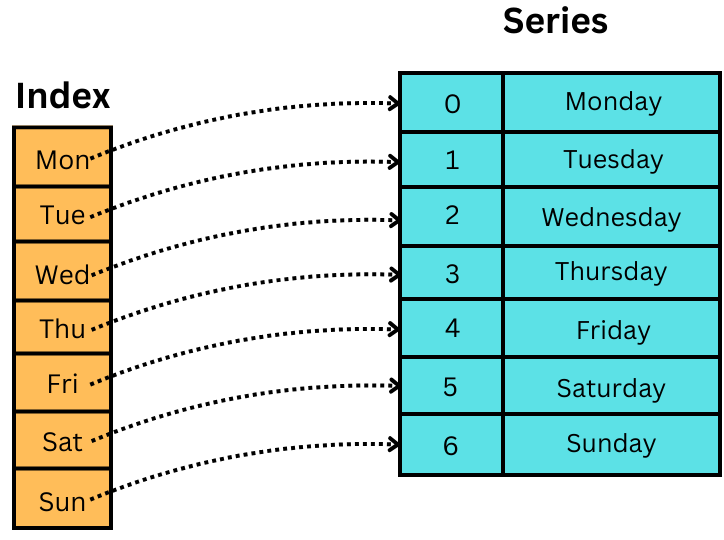
\includegraphics[scale=0.4]{img/Series}
\end{figure}

\subsection{Dataframe}

Dataframe is a two-dimensional tabular data structure.
A good way to look at a Dataframe is to see it as a Dictionary, where the keys are names of the columns of a table
and values are Series representing the columns themselves.
This also means that the Dataframe supports indexing of columns based on column names and integer-based indexing of rows.
Listing~\ref{lst:dataframe_basics} shows basic work with the Dataframe in Pandas.

\begin{lstlisting}[caption=Working with Dataframe in Pandas, label={lst:dataframe_basics}, captionpos=b]
import pandas as pd

# Create a Dataframe from a map of columns
data = {"column1": [1, 2, 3], "column2": ['a', 'b', 'c']}
dataframe = pd.DataFrame(data)

# Add a new row
dataframe.loc[3] = [4, 'd']

# Add a new column
dataframe['column3'] = [True, False, True, False]

# Replace a value
dataframe.at[1, 'column3'] = True
\end{lstlisting}

The Dataframe can also have an index associated with the rows of Series.
Consequently, the Dataframe supports Dictionary interface on both rows and columns.
Adding of new columns and rows is also supported.
The listing~\ref{lst:dataframe_index} shows how we can use indexes when working with Dataframes in Pandas.

\begin{lstlisting}[caption=Index on a Dataframe, label={lst:dataframe_index}, captionpos=b]
import pandas as pd

# Create a dataframe with index
dataframe = pd.DataFrame({
    'A': [1, 2, 3],
    'B': [4, 5, 6],
    'C': [7, 8, 9]
}, index=['x', 'y', 'z'])

# Access elements via index
print(dataframe.at['x', 'A']) # Prints 1

# Change value using index
dataframe.at['z', 'C'] = -9
\end{lstlisting}

The explanatory visualization of a Dataframe can be found in the Figure~\ref{fig:dataframe_schema}

\begin{figure}[H]
    \caption{Schema of a Dataframe}
    \label{fig:dataframe_schema}
    \centering
    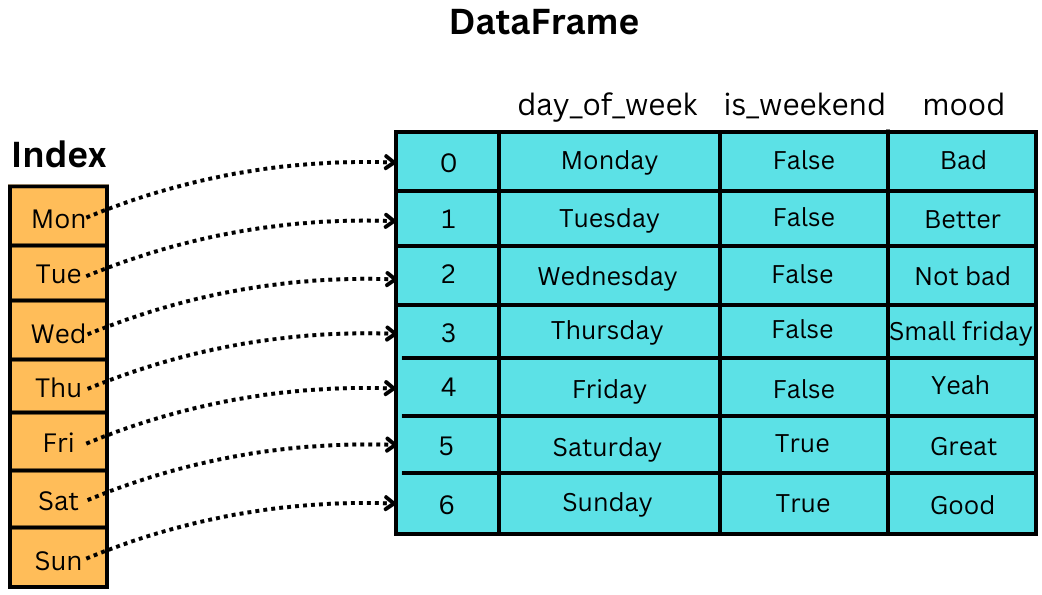
\includegraphics[scale=0.4]{img/Dataframe}
\end{figure}

The Dataframe is usually loaded from a CSV file via the \verb|read_csv| function, and the Dataframe that is the result
of the computation is usually stored to another CSV file via the \verb|to_csv| function.


\section{Common operations} %==========================================================================================%

To actually manipulate the data into some useful form, we need operations that are more powerful than just indexing and
adding and removing elements.
The operations that are commonly used in data manipulation were greatly influenced by the operations on relational
databases and the SQL language.
However, they are usually more flexible and customizable.

\subsection{Relational operations}

All well-known SQL relational databases support the following operations:
\texttt{SELECT, GROUP BY, HAVING, WHERE, JOIN, ORDER BY, AS}.
\\All these operations are also (usually under a different name) present in the data manipulation libraries as well.
We go through these operations and discuss their counterparts in Pandas.

\paragraph{SELECT} \leavevmode \\

The SELECT statement in SQL serves to select a specific subset of columns of a table.
In Pandas the square-brackets operator is used for that purpose.
As listing~\ref{lst:pandas_select} shows, the operator can return a Series or a Dataframe depending on whether
the argument is just a string or a list of strings.

\begin{lstlisting}[caption=Select in Pandas, label={lst:pandas_select}, captionpos=b]
dataframe = ... # initial dataframe

# Select a subset of columns (returns a dataframe)
subset = dataframe[["column1", "column3"]]

# Select one column (returns a Series)
column = dataframe["column2"]
\end{lstlisting}

Alternatively, the filter function can be also used for this purpose.
The important information for us will be that the operation returns a Dataframe with a different column structure
than the input Dataframe---it removes non-specified columns.

The SELECT statement in SQL can also do more than just selecting a subset of columns.
It can also apply aggregating function when used with group by.
This option is covered later when we talk about the GROUP BY operation.

\paragraph{WHERE} \leavevmode \\

The WHERE statement in SQL filters out the rows that do not match a given predicate.
In this case, Pandas was also able to make use of the square-brackets operator.
This time the operator accepts a Series of bool values and uses just the columns of a Dataframe with index the same as
some True value in the Series.
The Series of bools is usually (but not necessarily) created using vectorized operations.
The listing~\ref{lst:pandas_where} shows the usage.

\begin{lstlisting}[caption=Where in Pandas, label={lst:pandas_where}, captionpos=b]
dataframe = ... # initial dataframe

# Select just rows where the "age" column is at least 18
adults = dataframe[dataframe["age"] >= 18]
\end{lstlisting}

The important information for us will be that the result of this operation is a Dataframe with the same column structure.

\paragraph{AS} \leavevmode \\

The AS keyword is used to rename a specific column.
Pandas also has this feature, although it is named differently.
The function is called rename, and it accepts a mapping from old column names to new column names.
The listing~\ref{lst:pandas_as} shows how the rename function can be used.

\begin{lstlisting}[caption=As in Pandas, label={lst:pandas_as}, captionpos=b]
dataframe = ... # initial dataframe

# Rename some of the columns
renamed_dataframe = dataframe.rename(
    columns={"column1": "col1", "column2": "col2"}
)
\end{lstlisting}

\paragraph{ORDER BY} \leavevmode \\

ORDER BY is used to sort the data by some columns.
Pandas can do the same using the sort\_values function.
The example usage can be seen in the listing~\ref{lst:pandas_orderby}

\begin{lstlisting}[caption=Order by in Pandas, label={lst:pandas_orderby}, captionpos=b]
dataframe = ... # initial dataframe

# Order the dataframe rows by the values of column
# 'surname' in the ascending order
sorted = dataframe.sort_values(by=["surname"], ascending=True)
\end{lstlisting}

Note that the operation does not change the column structure of the Dataframe.

\paragraph{JOIN} \leavevmode \\

Join operation is used to combine rows from two tables based on some related columns.
There are four types of join---inner, left, right and outer.
Inner join returns rows that have matching rows in both tables.
Left join returns all rows from the left table and all matched rows from the right table.
Right join returns all rows from the right table and all matched rows from the left table.
And outer join returns rows where there is a match in either of the tables.

Pandas has a function called merge for this purpose.
It accepts two Dataframes and returns their corresponding join.
Besides the already mentioned joins, merge also supports a cross-join, which is essentially a cartesian product of
two sets of rows.
The listing~\ref{lst:pandas_join} shows how the merge function can be used as well as what parameters does the
function accept.

\begin{lstlisting}[caption=Join in Pandas, label={lst:pandas_join}, captionpos=b]
dataframe1 = ... # 1st initial dataframe
dataframe2 = ... # 2nd initial dataframe

inner = pd.merge(
    dataframe1, dataframe2, how="inner",
    left_on="left_key", right_on="right_key")
left = pd.merge(
    dataframe1, dataframe2, how="left", on="common_key")
right = pd.merge(
    dataframe1, dataframe2, how="right", on="common_key")
outer = pd.merge(
    dataframe1, dataframe2, how="outer",
    left_on="left_key", right_on="right_key"
cross = pd.merge(
    dataframe1, dataframe2, how="cross")
\end{lstlisting}

\paragraph{GROUP BY} \leavevmode \\

The group by operation aggregates the rows based on specified columns.
It does not return normal rows but summary rows, which we can apply aggregate functions on.
A Good example of an aggregate function can be max, min or sum.

Pandas has a function with the same name---groupby.
The function returns a DataframeGroupBy object, which we can apply aggregate functions on.
The listing~\ref{lst:pandas_groupby} shows the usage

\begin{lstlisting}[caption=Group by in Pandas, label={lst:pandas_groupby}, captionpos=b]
dataframe = ... # initial dataframe

# Group the dataframe by agg_column and return
# the mean of the "salary" column
dataframe.groupby(by=["work_department"])["salary"].mean()
\end{lstlisting}

\paragraph{HAVING} \leavevmode \\

Having operation works somewhat like a where operation on a summary rows---where group by was already applied.
In having clause, we can use any aggregate function in a predicate and then filter the summary rows based on such
predicate.

In Pandas, this can be done in many ways, but the usual one involves the filter function and lambdas.
Example of such usage is shown in the listing~\ref{lst:pandas_having}.

\begin{lstlisting}[caption=Having in Pandas, label={lst:pandas_having}, captionpos=b]
dataframe = ... # initial dataframe

# Group the dataframe by agg_column and return
# the columns that are in a work_department
# with an average salary higher than 10 000
dataframe \
    .groupby(by=["work_department"]) \
    .filter(lambda x: x["salary"].mean() > 10000)
\end{lstlisting}


\subsection{Vectorized operations}

When we discussed the SQL WHERE clause, we came across the following line of code:

\verb|adults = dataframe[dataframe["age"] >= 18]|

We said that this line of code filters out the rows where the age is less than 18.
We also said that the square-bracket operator accepts a Series of bools.
So the expression~\verb|dataframe["age"] >= 18]| must return a Series of bools.
But why does this work?
How can we compare a Series to a number?

In Pandas, the Series can be summed, subtracted, multiplied or compared with values that are either Series or a scalar
values.
The listing~\ref{lst:vectorized_operations} shows the behavior of some vectorized operations in Pandas performed in
the interactive mode.

\begin{lstlisting}[caption=Vectorized operations, label={lst:vectorized_operations}, captionpos=b]
>>> sr1 = pd.Series([1, 2, 3])
>>> sr1 + 7
0     8
1     9
2    10
dtype: int64
>>> 3 * sr1
0    3
1    6
2    9
dtype: int64
>>> sr1 / sr1
0    1.0
1    1.0
2    1.0
dtype: float64
>>> sr2 = pd.Series(["a", "b", "c"])
>>> sr2 * 2
0    aa
1    bb
2    cc
dtype: object
>>> sr2 + "x"
0    ax
1    bx
2    cx
dtype: object
\end{lstlisting}

\section*{Summary} %===================================================================================================%
\addcontentsline{toc}{section}{Summary}

We covered two common data structure interfaces used in data analysis - Series and Dataframe.
Series is a one-dimensional List-like data structure with support for index and an axis label.
Data frame is a two-dimensional structure---a dictionary of columns.
The whole Dataframe can have an index associated, and the column of a Dataframe can be seen as a Series.
Many operations in the data manipulation libraries are influenced by the SQL language operations such as join, select,
group by, where, order by etc.
The data structures also support vectorized operations like sums, products or comparing.

All discussed topics were demonstrated on Pandas code snippets.
However, the Pandas library is a large project and the goal of this chapter was not to explore it all.
More detailed information can be found in the API reference of Pandas\cite{pandas_docs}.


\chapter*{Conclusion}
\addcontentsline{toc}{chapter}{Conclusion}

The aim of this thesis was to design and implement a code-analysis tool for the Pandas library that would be capable of
checking common kinds of errors such as accesses to misspelled or non-existent columns.
The resulting system should have been evaluated through a set of realistic case studies.
Let us recap and summarize to what extent we did that.

We first defined a framework for the Abstract Interpretation analysis of the Dataframe and Series type and then expanded it
to other types such as strings, numbers, lists, etc.
Then we used the framework to implement the Pandalyzer.
The Pandalyzer is a code-analysis tool that uses Abstract Interpretation to interpret Python code with Pandas
library.
The Pandalyzer is capable of detecting errors such as access to non-existent column, operation on incompatible types,
incorrect function arguments, operations leading to an incorrect state.
It also reports the structure of the output CSV files and is able to accept information about the structure of the input CSV files.
The Pandalyzer is able to work with some amount of uncertainty generated from the user input.
The supported functions include merge, groupby, drop, rename, read\_csv, to\_csv, concat, Dataframe creation,
Series creation, the subscript operator in both get and set contexts and vectorized sums and products, aggregation function
such as mean, sum, first, last, count or head.
As shown in the case studies in the chapter~\ref{ch:evaluation-of-solution}, this set of functions already gives
the user enough flexibility to do many various data manipulation tasks.
Moreover, the Pandalyzer is highly extensible, so implementing support for other Pandas functions is possible.

On the other hand, the Pandalyzer has some limitations.
It now only supports a subset of Python language so the analyzer will not be able to proceed with the analysis when
it encounters unknown Python construct.
However, it is planned in the Future Work~\ref{sec:future-work} to add support for the rest of the Python language.

\section*{Related Work}
\addcontentsline{toc}{section}{Related Work}

The idea to use Abstract Interpretation to analyze programs working with Dataframes was already proposed by~Yungyu~Zhuang
and~Ming-Yang~Lu~\cite{Zhuang:2022:TypeChecking}.
They also created a proof of concept implementation named PDChecker.
However, PDChecker does not have as many checks, does not report output CSV files (via to\_csv() function) and
does not allow for interpreting multiple branches of if-statements and other sources of non-determinism.

Another related subject are the type hints~\cite{python_typing} in Python language.
The language itself does not enforce any typing rules, but we can put type annotations in the code and analyzers
integrated in the IDE can warn us in case that the types do not match.
Unfortunately, this is not useful for our case, since the type annotations are only able to express that
(for example) the function returns a Pandas Dataframe, not a Pandas Dataframe with a specific column structure.

The Types for Tables~\cite{types_for_tables} article defines the Table API - the definition of a table and operations on
a table similarly as we did it in the chapter~\ref{ch:putting-it-all-together}.


\section*{Future Work}\label{sec:future-work}
\addcontentsline{toc}{section}{Future Work}

There is a lot of plans ahead of us regarding the implementation.
In the future, we would like to support more Pandas operations since Pandas is a large library with many useful
operations.
We would also like to add support for working with Indexes on Dataframes and Series.
The Pandalyzer so far supports a limited subset of Python language constructs.
We chose the most useful language constructs for the data manipulation.
However, the plan for the future is to add support for other Python constructs such as Lambdas, Match statements,
For-loops or Classes.
As of now, Pandalyzer is only able to analyze one module, so extending it to be able to analyze multiple modules together
could be also a useful extension.

The Pandalyzer tool could be also extended for other related Python libraries.
A good example is the numpy library for working with vectors, matrices etc.
The abstraction could be defined as the dimensions of the vectors and matrices.
Another good example of a library worth including to the Pandalyzer is the matplotlib library for data visualization.
We could support reporting of what visualizations would be displayed to the user.
This could be implemented in a similar way as the analysis of the to\_csv function in Pandas.

Another field where the Pandalyzer could be extended is its integration to the IDEs such as PyCharm or VS Code.
This could be done using the Language Server Protocol.

%%% Bibliography
%%% Bibliography (literature used as a source)
%%%
%%% We employ biblatex to construct the bibliography. It processes
%%% citations in the text (e.g., the \cite{...} macro) and looks up
%%% relevant entries in the bibliography.bib file.
%%%
%%% See also biblatex settings in thesis.tex.

%%% Generate the bibliography. Beware that if you cited no works,
%%% the empty list will be omitted completely.

% We let bibliography items stick out of the right margin a little
\def\bibfont{\hfuzz=2pt}

\printbibliography[heading=bibintoc]

%%% If case you prefer to write the bibliography manually (without biblatex),
%%% you can use the following. Please follow the ISO 690 standard and
%%% citation conventions of your field of research.

% \begin{thebibliography}{99}
%
% \bibitem{lamport94}
%   {\sc Lamport,} Leslie.
%   \emph{\LaTeX: A Document Preparation System}.
%   2nd edition.
%   Massachusetts: Addison Wesley, 1994.
%   ISBN 0-201-52983-1.
%
% \end{thebibliography}


%%% Figures used in the thesis (consider if this is needed)
\listoffigures

%%% Tables used in the thesis (consider if this is needed)
%%% In mathematical theses, it could be better to move the list of tables to the beginning of the thesis.
\listoftables

%%% Abbreviations used in the thesis, if any, including their explanation
%%% In mathematical theses, it could be better to move the list of abbreviations to the beginning of the thesis.
\chapwithtoc{List of Abbreviations}

%%% Attachments to the bachelor thesis, if any. Each attachment must be
%%% referred to at least once from the text of the thesis. Attachments
%%% are numbered.
%%%
%%% The printed version should preferably contain attachments, which can be
%%% read (additional tables and charts, supplementary text, examples of
%%% program output, etc.). The electronic version is more suited for attachments
%%% which will likely be used in an electronic form rather than read (program
%%% source code, data files, interactive charts, etc.). Electronic attachments
%%% should be uploaded to SIS and optionally also included in the thesis on a~CD/DVD.
%%% Allowed file formats are specified in provision of the rector no. 72/2017.
\appendix
\chapter{Attachments}

\section{First Attachment}

\openright
\end{document}
